% !TEX root = ../../../main.tex
% 来源：中学数学实验教材·第一册（代数）
% 章节：因式分解与余式定理 / 余式定理及其推论
% 原始文件：5.tex，行 1673-1698
% 类型：tikz
% ---
    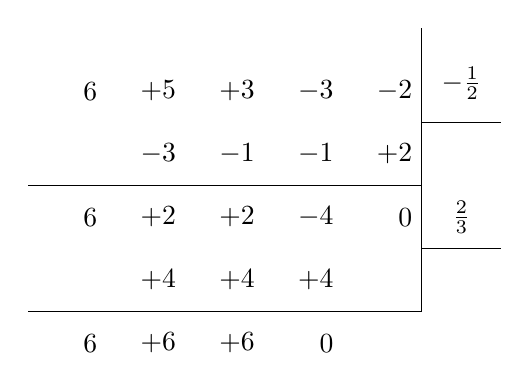
\begin{tikzpicture}
\foreach \x/\xtext in {0/6,1/+6,2/+6,3/\boxed{0}}
{
    \node at  (\x,0)[left]{$\xtext$};
}        
\foreach \x/\xtext in {1/+4,2/+4,3/+4}
{
    \node at  (\x,.8)[left]{$\xtext$};
}  
\foreach \x/\xtext in {0/6,1/+2,2/+2,3/-4, 4/\boxed{0}}
{
    \node at  (\x,1.6)[left]{$\xtext$};
}  
\foreach \x/\xtext in {1/-3,2/-1,3/-1, 4/+2}
{
    \node at  (\x,2.4)[left]{$\xtext$};
}  
\foreach \x/\xtext in {0/6,1/+5,2/+3,3/-3, 4/-2}
{
    \node at  (\x,3.2)[left]{$\xtext$};
}  
\draw (-1,.4)--(4,.4);  \draw (-1,2)--(4,2);\draw(4,.4)--(4,4);
\node at (4.5,3.3){$-\frac{1}{2}$};
\node at (4.5,1.6){$\frac{2}{3}$};
\draw (4,1.2)--(5,1.2); \draw (4,2.8)--(5,2.8);
 \end{tikzpicture}    
